%% 
%% Copyright 2007, 2008, 2009 Elsevier Ltd
%% 
%% This file is part of the 'Elsarticle Bundle'.
%% ---------------------------------------------
%% 
%% It may be distributed under the conditions of the LaTeX Project Public
%% License, either version 1.2 of this license or (at your option) any
%% later version.  The latest version of this license is in
%%    http://www.latex-project.org/lppl.txt
%% and version 1.2 or later is part of all distributions of LaTeX
%% version 1999/12/01 or later.
%% 
%% The list of all files belonging to the 'Elsarticle Bundle' is
%% given in the file `manifest.txt'.
%% 

%% Template article for Elsevier's document class `elsarticle'
%% with numbered style bibliographic references
%% SP 2008/03/01

\documentclass[preprint,12pt, a4paper]{elsarticle}

%% Use the option review to obtain double line spacing
%% \documentclass[authoryear,preprint,review,12pt]{elsarticle}

%% For including figures, graphicx.sty has been loaded in
%% elsarticle.cls. If you prefer to use the old commands
%% please give \usepackage{epsfig}

%% The amssymb package provides various useful mathematical symbols
\usepackage{amssymb}
%% The amsthm package provides extended theorem environments
%% \usepackage{amsthm}

%% The lineno packages adds line numbers. Start line numbering with
%% \begin{linenumbers}, end it with \end{linenumbers}. Or switch it on
%% for the whole article with \linenumbers.
\usepackage{lineno}

\usepackage{float}
\restylefloat{table}

\journal{SoftwareX}

\begin{document}

\begin{frontmatter}

%% Title, authors and addresses

%% use the tnoteref command within \title for footnotes;
%% use the tnotetext command for theassociated footnote;
%% use the fnref command within \author or \address for footnotes;
%% use the fntext command for theassociated footnote;
%% use the corref command within \author for corresponding author footnotes;
%% use the cortext command for theassociated footnote;
%% use the ead command for the email address,
%% and the form \ead[url] for the home page:
%% \title{Title\tnoteref{label1}}
%% \tnotetext[label1]{}
%% \author{Name\corref{cor1}\fnref{label2}}
%% \ead{email address}
%% \ead[url]{home page}
%% \fntext[label2]{}
%% \cortext[cor1]{}
%% \address{Address\fnref{label3}}
%% \fntext[label3]{}

\title{RadLib: a radiative heat transfer model library for CFD}

%% use optional labels to link authors explicitly to addresses:
%% \author[label1,label2]{}
%% \address[label1]{}
%% \address[label2]{}

%\renewcommand{\thefootnote}{\fnsymbol{footnote}}
\author{Victoria B. Stephens}
\author{Sally Jensen}
\author{David O. Lignell\corref{cor1}}

\cortext[cor1]{Corresponding author. \ead{davidlignell@byu.edu}}

\address{Department of Chemical Engineering, Brigham Young University, Provo, UT 84602, United States}

\begin{abstract}
%% Text of abstract 
Ca. 100 words
\end{abstract}

\begin{keyword}
%% keywords here, in the form: keyword \sep keyword
radiative heat transfer \sep reacting flows  \sep CFD
\end{keyword}

\end{frontmatter}

\section*{Required Metadata}
\label{}

\section*{Current code version}
\label{}

Ancillary data table required for subversion of the codebase. Kindly replace examples in right column with the correct information about your current code, and leave the left column as it is.

\begin{table}[H]
\begin{tabular}{|l|p{6.5cm}|p{6.5cm}|}
\hline
\textbf{Nr.} & \textbf{Code metadata description} & \textbf{Please fill in this column} \\
\hline
C1 & Current code version & TODO 2.1 \\
\hline
C2 & Permanent link to code/repository used for this code version & $github.com/BYUignite/RadLib$ \\
\hline
C3 & Code Ocean compute capsule & N/A \\
\hline
C4 & Legal Code License   & MIT license (MIT) \\
\hline
C5 & Code versioning system used & Git \\
\hline
C6 & Software code languages, tools, and services used & C++, Python 3 \\
\hline
C7 & Compilation requirements, operating environments \& dependencies & TODO \\
\hline
C8 & If available Link to developer documentation/manual & TODO \\
\hline
C9 & Support email for questions & davidlignell@byu.edu \\
\hline
\end{tabular}
\caption{Code metadata (mandatory)}
\label{} 
\end{table}


\linenumbers

% TO DO
% - update README
% - tag software version
% - decide on and generate documentation

\section{Motivation and significance}
\label{s:motivation}

% Brain dump for first draft
Why did we make this? Radiation is hard to deal with in CFD. It's complicated. You can't really get analytic solutions to practical problems. In lots of cases, that's fine because radiation can be safely neglected; it's not usually the dominant mode of heat transfer. However, we do combustion CFD. Radiation isn't always important to combustion problems, but when it is, simulations can get grossly inaccurate. So we need a nice way to account for radiation in our CFD simulations. 

When is radiation important to combustion simulations? In high-temperature systems, radiation can often be neglected in the beginning and middle of the simulation (assuming, say, a jet flame or a counterflow flame or something like that). At those times (which I'm going to call "early flame"), convective heat transfer dominates pretty heavily. However, radiation becomes more important for late-stage flame phenomena, either after some time has gone by (radiation time scales?), or physically high up in a flame where convection doesn't dominate as much as below, or just in areas that are relatively far away from the flame sheet itself where the reactions are happening. There's also soot, which involves radiation heavily, but soot particles are so big and slow that their time and length scales (and their radiative time scales) mean that radiation doesn't become important until late in the flame evolution. 

So what's the problem? Why hasn't this been done already? Radiation is complicated. So is combustion. Combustion in particular can be so complex that direct simulations are too computationally expensive for us to simulate configurations that are practical for engineering systems. Direct simulations are usually used as a research tool. Other modeling approaches exist (LES, ODT, etc.) that lower the computational cost and allow us to simulate practical things. So far so good. 

Radiation is a little like combustion in that its core mechanisms are complex, physically and mathematically. In addition, it's directional AND depends on the wavelength of the energy involved (other heat transfer doesn't have the wavelength dependence); its governing equations integrate over direction and wavelength, which makes things extra complicated. RADIATION GOVERNING EQUATIONS HERE.  Convective heat transfer follows easy rules, but radiation doesn't. There are simple systems in which we can boil things down to analytic solutions, but most of the time, the simple equations don't apply, and that's often true in combustion systems where there are so many different length and time scales involved. The fundamental equations of radiative heat transfer are big and mathematically complex; they don't have analytic solutions except in the simplest geometries. So what do we do? One of two things. One, we do ray tracing (sometimes referred to as Monte Carlo simulations. These can be extremely accurate, but super computationally expensive. Essentially the equivalent of a direct numerical solution. Two, we simplify the the equations. We make assumptions. And so on. This is potentially less accurate, but more practical. By simplifying the fundamental governing equations, we create models that apply to various situations, systems, and geometries (i.e. black body assumptions, directional assumptions, etc.). There are models developed for CFD and specific combustion systems. These are the models that we've put into practice here in such a way that they're easy to apply to various systems. Modular organization for this purpose.

So far there isn't an easy way to access and use radiation models. There are simple ones in Cantera (check this, there might not be any), but they make too many assumptions or don't work well for combustion or what have you. RadLib is a radiation library of models that you can apply to any simulation type, and we'd like to add it to Cantera, too. Basically, there isn't a reliable way to do radiation calculations in CFD simulations without coding the models yourself, which is extra hard because they're complicated and hard. So we've done it for you and put them in a library that easy for anyone to use.

Models we're using:
\begin{itemize}
 \item planck mean (optically thin?) with coefficients from TNF website \cite{Smith_2003}
 \begin{itemize}
  \item other references from TNF website: \cite{Grosshandler_1993,Frank_2000,Zhu_2002,Barlow_2001}
 \end{itemize}
 \item weighted sum of grey gases \cite{Bordbar_2014,Bordbar_2020}
 \item RCSLW model \cite{Solovjov_2017}
 \begin{itemize}
  \item SLW model \cite{Solovjov_2001}
  \item LCSLW \cite{Solovjov_2020}
  \item "It is shown that the Rank Correlated SLW model is the most robust of all models, and demonstrates that it can achieve accurate solutions with as few as 3–5 gray gases." \cite{Badger_2019}

 \end{itemize}  
\end{itemize}
Discuss pros and cons of each model for combustion simulations? You still have to pick the right one for your simulation and situation. That discussion might fit better in software description section. See example section for comparisons of models. 

%Author guidelines for this section:
%\begin{itemize}
% \item Introduce the scientific background and the motivation for developing the software. 
% \item Explain why the software is important, and describe the exact (scientific) problem(s) it solves.
% \item Indicate in what way the software has contributed (or how it will contribute in the future) to the process of scientific discovery; if available, this is to be supported by citing a research paper using the software.
% \item Provide a description of the experimental setting (how does the user use the software?).
% \item Introduce related work in literature (cite or list algorithms used, other software etc.).
%\end{itemize}

\section{Software description}
\label{s:description}

%Author guidelines for this section
%\begin{itemize}
% \item Describe the software in as much as is necessary to establish a vocabulary needed to explain its impact.
% \item  Give a short overview of the overall software architecture; provide a pictorial component overview or similar (if possible). If necessary provide implementation details.
% \item Present the major functionalities of the software.
%\end{itemize}

\subsection{Model descriptions}
\label{s:models}

RadLib includes three models of varying complexity and accuracy to calculate the radiation absorption coefficients and their weighting factors for each gas considered by the model. Radiation absorption coefficients are typically calculated using correlations relating them local properties such as temperature, total pressure, or species partial pressure, depending on the model. Correlations come from curve fits to high-resolution radiation property databases. At present, RadLib considers up to four gas species (H$_2$O, CO, CO$_2$, and CH$_4$) and, optionally, soot volume fraction in its calculation of absorption coefficients and weighting factors. 

Once the radiative absorption coefficients are calculated, they are then used to solve the radiative transfer equation (RTE), which depends on the simulation configuration and assumptions. Solving the RTE is not the focus of this software, but RadLib's example cases do employ a simple implicit trapezoid method solver to calculate the radiative heat flux and volumetric heat source profiles between two parallel planes. [MORE DESCRIPTION OF SOLVER GOES HERE?]

[OTHER THINGS THAT APPLY TO ALL MODELS GO HERE]

[MAYBE INCLUDE SOME BASIC INFO ON LBL?]

\subsubsection{Planck Mean absorption coefficients}
\label{s:planckmean}

When we refer to the Plank Mean model, what we're using is actually the Planck Mean (PM) absorption coefficients, calculated from the correlations given on the TNF workshop site \citep{Smith_2003}. Their correlations (temperature dependent) are based on the RADCAL model in \citep{Grosshandler_1993}. The TNF radiation model is also documented in \citep{Barlow_2001}.

This model is commonly used because it's relatively simple, easy to implement, low in computational expense, and provides reasonably accurate results in many cases. 

Quote from TNF site page: "The characteristics of some flames selected for the workshop are such that a model based upon the assumption of optically thin radiative heat loss should yield reasonable accuracy. This has been demonstrated for the simple hydrogen jet flames \cite{Barlow_1999}. However, there is some evidence that the optically thin model significantly over predicts radiative losses from the CH4 flames in the TNF library, due to strong absorption by the 4.3-micron band of CO2 \cite{Frank_2000,Zhu_2002,Coelho_2002}." Basically, it works well for flames that are actually optically thin, but not so well for flames that aren't. This is especially true of sooting flames. 

\subsubsection{Weighted sum of gray gases (WSGG)}
\label{s:wsgg}
The basic assumption of weighted sum of gray gases (WSGG) models in general is that the non-gray behavior of gas mixtures, in this case H$_2$O and CO$_2$, can be modeled by a weighted sum of several gray gases and one transparent gas (which represents the spectral windows between absorption bands). 
RadLib uses the WSGG model presented by Bordbar et al. \citep{Bordbar_2014,Bordbar_2020}, which uses correlations based on the HITEMP 2010 database \cite{Rothman_2010}. RadLib, in accordance with the Bordbar et al. WSGG method cited above, uses a mixture of four gray gases and one transparent gas. Absorption coefficients are calculated by 
\begin{equation}
 K_i=\sum_{k=0}^{4}d_{i,k}M_r^k,
\end{equation}
where $K_i$ is the absorption coefficient for species $i$, $d_{i,k}$ is a species-specific correlated model coefficient, and $M_r$ is the molar ratio $Y_{\mathrm{H_2O}}/Y_{\mathrm{CO_2}}$. The weight factors are calculated by 
\begin{equation}
 a_i=\sum_{j=0}^{4}b_{i,j}T_r^j,
\end{equation}
where $a_i$ is the weighting factor for species $i$ and $T_r$ is a normalized temperature equal to $T/T_{ref}$ with $T_{ref}=1200$K. The value of $b_{i,j}$ is calculated by 
\begin{equation}
 b_{i,j}=\sum_{k=0}^{4}C_{i,j}M_r^k,
\end{equation}
where $C_{i,j}$ is another correlated model coefficient and $M_r$ is the molar ratio $Y_{\mathrm{H_2O}}/Y_{\mathrm{CO_2}}$ as above. 

\subsubsection{Rank Correlated SLW (RCSLW) model}
\label{s:RCSLW}

\subsection{Software Architecture}
\label{s:architechture}

RadLib is an object-oriented C++ class library. 

Examples folder contains sample driver scripts for using the library. 

Python version somewhere? Corresponding examples?

%%%%%%%%%%%%%%%%%%%%%%%%%%%%%%%%%%%%%%%%%%%%%%%%%%%%%%%%%%%%%%%%%%%%%%%%%%%%%%%%

\section{Illustrative Examples}
\label{s:Examples}

Several examples are presented to illustrate the behavior of the models. The examples show heat flux $q$ or volumetric heat source $Q$ one one-dimensional configurations with varying gas compositions and temperatures. We compare the PM, WSGG, and RCSLW models for each example. The examples are taken from those presented by Solvojov et al., (2017) \cite{Solovjov_2017}, and Bordbar et al., 2020 \cite{Bordbar_2020}; the number corresponds to the example in the respective referece. A ray-tracing code is used to solve the radiative transport equation between two parallel plates. 
Table~\ref{t:examples} summarizes the cases. Example S1 is a hot slab next to a cold slab where the cold thickness varies; Example S2 is similar but isothermal with a \emph{thick} slab of high CO$_2$ next to a \emph{thin} slab of low CO$_2$ of varying thickness; Example S3 has parabolic temperature and H$_2$O profiles; Example S4 has a triangular temperature profile between equally-spaced isothermal regions; Example S5 is a half-sinusoid decreasing in temperature from 1500 to 500 K; and Example B3 has symmetric temperature and H$_2$O profiles with central peaks of 1800 K and 1, respectively (with $y_{CO2}=1-y_{H2O}$). In each case, comparison is made to the line-by-line (LBL) data presented in the references. 
%
\begin{table}
    \caption{Summary of example cases presented. S1-S5 are from \cite{Solovjov_2017}; B3 is from \cite{Bordbar_2017}. All cases have $P=1$ atm, black walls.}
    \label{t:examples}
    \centering
    \resizebox{\textwidth}{!}{
    \begin{tabular}{c l l c c c}
        \hline
        Example & T(K)                           & $y_{H2O}$  $y_{CO2}$ (mole frac.)                     & L (m)   & $T_{walls}$ (K)\\
        \hline
        S1 & $T(x<0.5)=2000$; $T(x>0.5)=300$     & $y_{CO2}=0.1$, $y_{H2O}=0.2$                          & 0.5-2.5 & cold, cold     \\
        S2 & T=1000                              & $y_{CO2}(x<0.5)=0.4$, $y_{CO2}(x>0.5)=0.1$            & 0.5-2.5 & cold, cold     \\
           &                                     & $y_{H2O}=0.0$                                         &         &                \\
        S3 & $T(x) = 4000x(L-x)/L^2 + 800$       & $y_{H2O}(x) = 0.8x(L-x)/L^2 + 0.12$                   & 1       & 800, 800       \\
           &                                     & $y_{CO2}=0$                                           &         &                \\
        S4 & middle third triangular to 2500     & $y_{H2O}=0.1$, $y_{CO2}=0$                            & 0.3     & 500, 500       \\
        S5 & $T(x) = 1000 + 500\cos(\pi x/L)$    & $y_{H2O}=0.1$, $y_{CO2}=0$                            & 2       & 1500, 500      \\
        B3 & $T(x) = 400 + 1400\sin(\pi x/L)^2$  & $y_{H2O}(x) = 0.0001 + 0.9999\sin(\pi x/L)^2$         & 1       & 400, 400       \\
           &                                     & $y_{CO2}=1-y_{H2O}$                                   &         &                \\
        \hline
    \end{tabular}
    }
\end{table}
%

The examples are provided with the radlib code and implemented in both C++ and Python. A Juptyer notebook is provided with the Python examples that runs the examples, displays the plots, and saves the plots to PDF files. Python and Cython versions of the one-dimensional solver \texttt{parallel\_planes} are provided for convenience.

These examples are not meant to be exhaustive, and details about the motivation of these examples and the behavior of the specific models is to be found in the respective references. The cases presented are intended to illustrate the use of the radiative library. While not shown  for brevity, the implemented WSGG and RCSLW models give essentially identical results to those presented in \cite{Solovjov_2017,Bordbar_2020}, so that these examples also serve as a validation of the implementation of the models.

Figure~\ref{f:examples} shows comparative results for the different radiation models for these cases. 
%
\begin{figure}
    \begin{center}
    \begin{tabular}{c c}
        Example S1 & Example S2 \\
        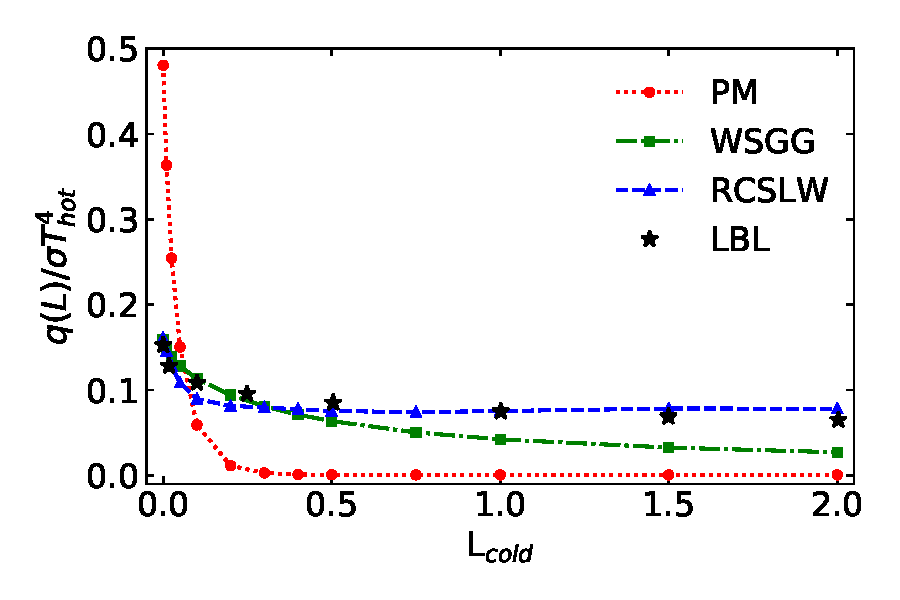
\includegraphics[width=3 in]{ex_1.pdf} &
        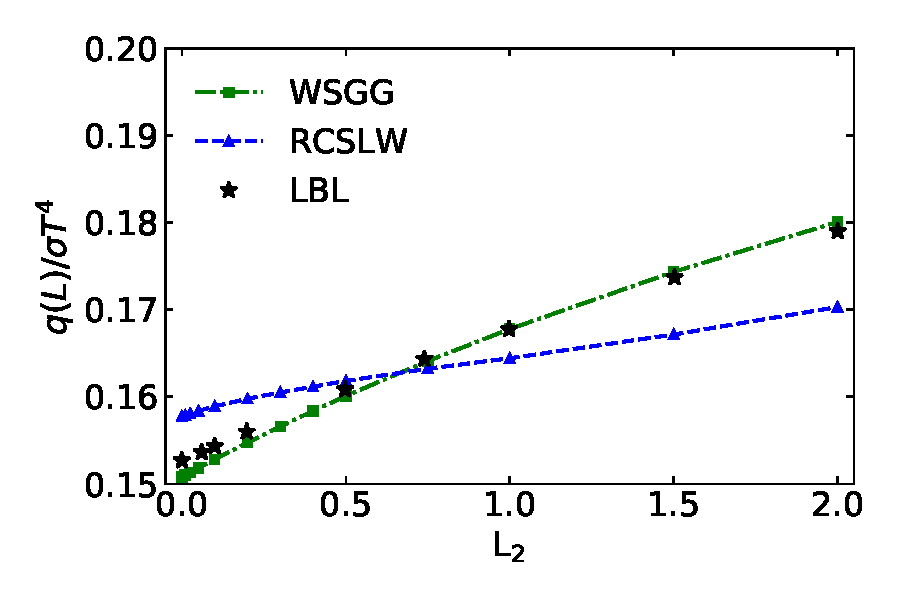
\includegraphics[width=3 in]{ex_2b.pdf} \\
        Example S3 & Example S4 \\
        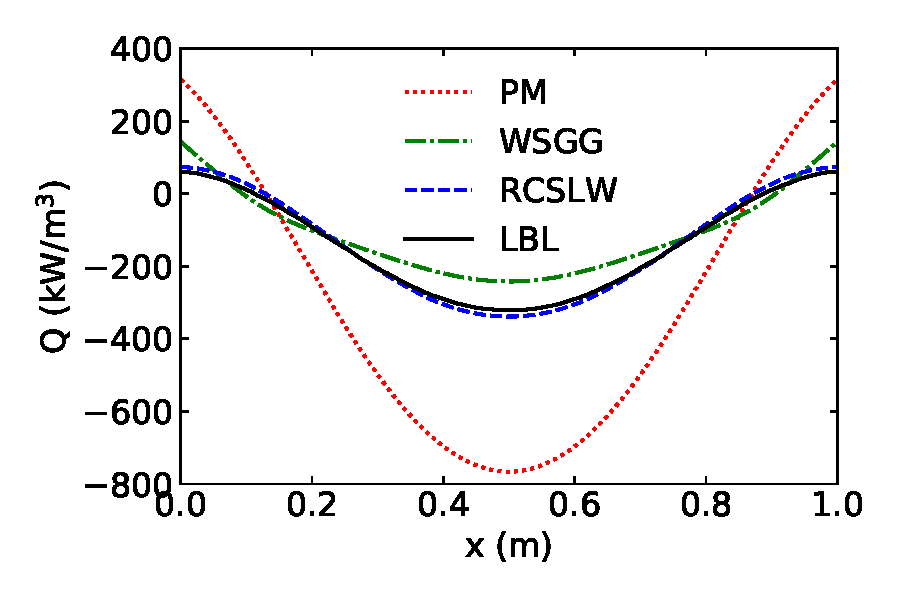
\includegraphics[width=3 in]{ex_3a.pdf} &
        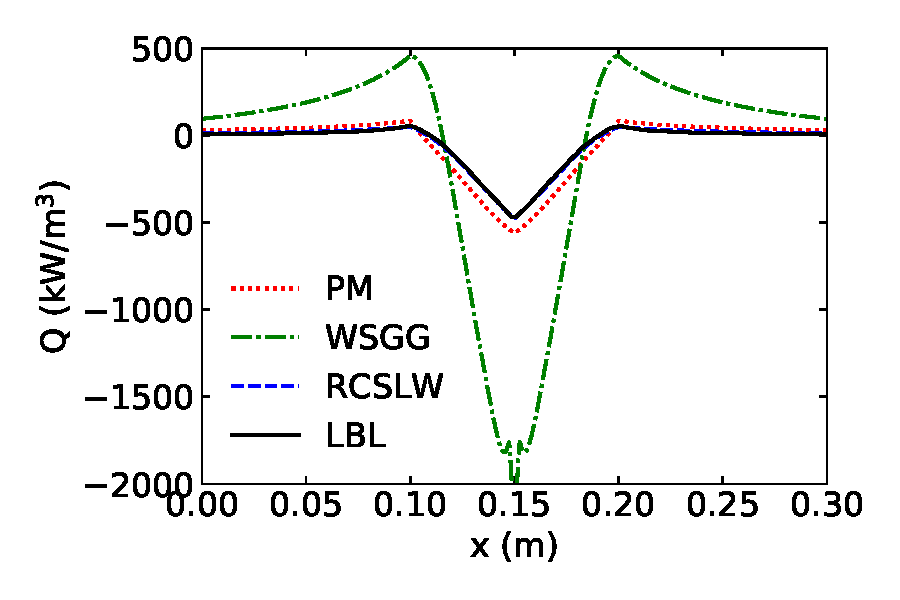
\includegraphics[width=3 in]{ex_4a.pdf} \\
        Example S5 & Example B3 \\
        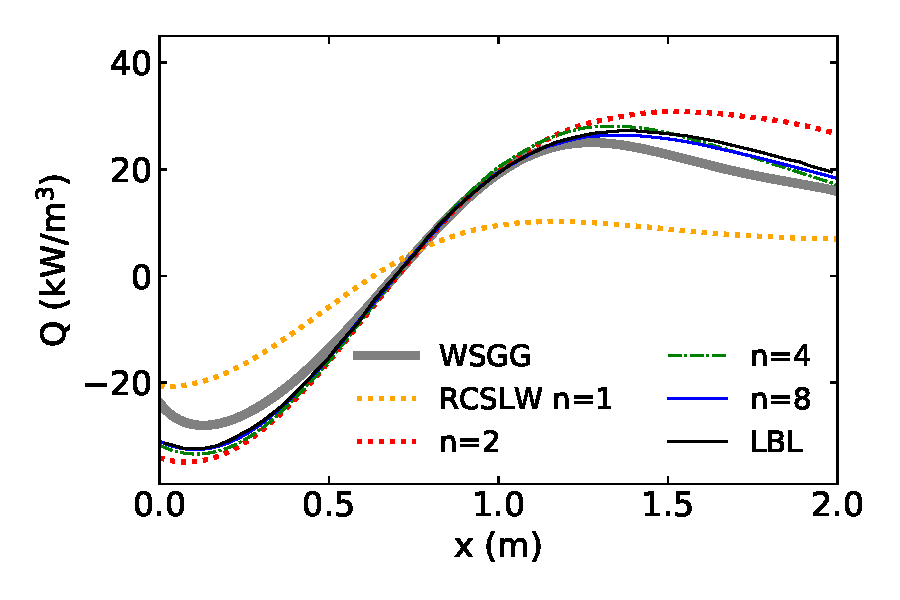
\includegraphics[width=3 in]{ex_5b.pdf} &
        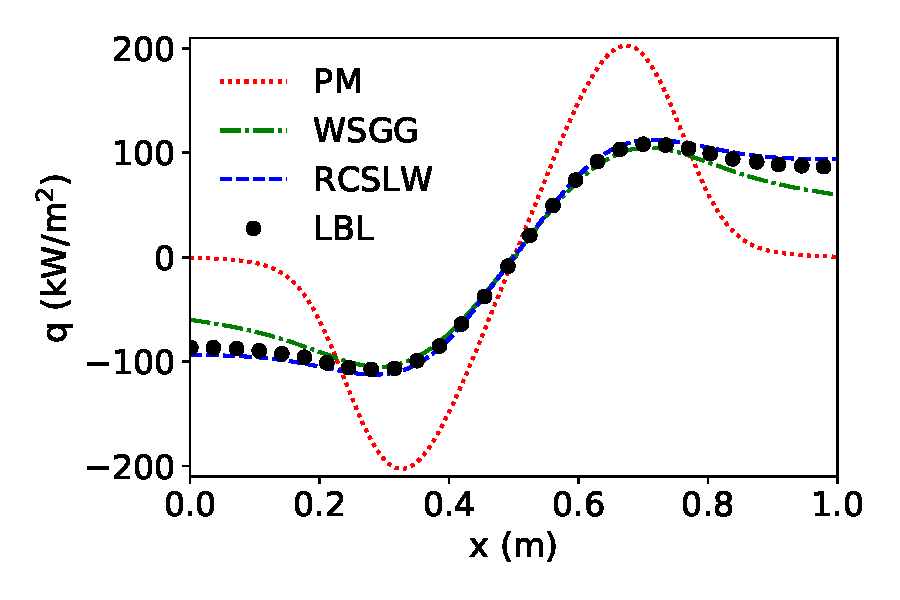
\includegraphics[width=3 in]{ex_6.pdf}
    \end{tabular}
    \caption{Results for examples summarized in Table~\ref{t:examples}.}
    \label{f:examples}
    \end{center}
\end{figure}
%
In general, the PM model performs poorly compared to the WSSGG and RCSLW models. A notable exception is Example S4. In Example S2, the PM $q(L)/\sigma T^4$ is off scale at an essentially constant at a value of unity. The PM absorption coefficient is 27.4 atm$^{-1}$m$^{-1}$, giving optical thicknesses of 0.09 and 0.36 m in the thick and thin layers, respectively, which are relatively small compared to the isothermal domain size greater than 0.5 m. Example S5 omits the PM model to more clealy show the behavior of the WSGG and RCSLW models. For that example, the PM values follow the shape of the other curves but $Q$ varies from around -80 at $x=0$ to a peak of 200 at x=$1.5$ m, and dropping to 100 kW/m$^3$ at $x=2$ m. In all examples, four gray ($n=4$) and one clear gas are computed for the RCSLW models to give a consistent comparison to the WSGG model. Example S5 shows the sensitivity of the RCSLW model to the number of gases used. When $n$ is increased to eight the RCSLW model improves to show nearly perfect agreement with the LBL data in Example S2.
In all Examples, the RCSLW model is initialized using the mean temperature and composition on the domain. In Example S5, the RCSLW model converges to the LBL solution when the model is initialized using the maximum temperature instead of the average temperature.

% TODO: do the cost comparison  <13-11-20, dol> %

%%%%%%%%%%%%%%%%%%%%%%%%%%%%%%%%%%%%%%%%%%%%%%%%%%%%%%%%%%%%%%%%%%%%%%%%%%%%%%%%

\section{Impact}
\label{s:impact}

As far as I'm aware, there isn't an easy way to incorporate radiative heat transfer into a CFD simulation. Most cases use optically thin assumption (which works in some cases, but not in others) or neglect radiation entirely (also applicable sometimes, but not always). [Refer to TNF website radiation page here.] Unfortunately, this means that when you simulation some configuration in which radiation might be important to the overall heat transfer, you won't get accurate simulation results. Furthermore, if your study is about something else entirely, your radiation model (or lack thereof) becomes a source of error that may be very difficult to separate from other sources of error in your simulation study (i.e. soot modeling studies). As of right now, if you want any detailed radiation treatment, you have to code it yourself, which is difficult and requires external validation. 

RadLib can make researchers' lives easier by providing a library of prevalidated radiation models that can be switched out with no difficulty. Additional models can be added easily using the provided modular framework. Researchers can even use Radlib as a tool for comparing models. No need to code multiple different complex radiation models yourself just to decide which one works best for your simulation. And no need to puzzle through the literature to figure our which model(s) might be best for your simulation, either; instead, you can test them yourself. It saves tons of time and effort that researchers can now put toward results rather than code or model development. 

By putting all these models side by side in a modular framework, RadLib also provides a structure on which new or altered radiation models can be tested against existing ones. Maybe more comparative studies can be done, especially for more complex simulation cases. We plan to add radiation models as appropriate to RadLib, too. 

RadLib opens up new horizons for CFD simulations, especially in combustion cases. It is designed such that it can be easily incorporated into existing research codes. Our group plans to use it with ODT [CITE OTHER SOFTWAREX PAPER HERE?] alongside soot model library (in development) to study late-flame phenomena such as soot oxidation, flame extinction, and soot-flame breakthrough. These topics in particular are difficult because they require accurate simulation data over a relatively long computational time in addition to good models for both soot chemistry (which is an active research area) and radiation heat transfer (which is the difficult part that RadLib can solve). Using RadLib for such studies allows us to separate and quantify sources of error that may occur due to various models, which is super difficult if you only have one model to work with or it hasn't been validated well. 

RadLib can also be used outside of combustion CFD research for anything involving radiative heat transfer. Potential research areas that could benefit include atmospheric and climate sciences, interstellar phenomena, improving efficiency of energy-producing processes, safety in chemical plant design, etc. We aren't experts in these areas, but radiative heat transfer is a universal phenomena that applies to any system or process that involves heat transfer. 

This software has not been used outside of the current research group, and it is not used in any commercial settings at this time. 

%Author guidelines for this section
%\begin{itemize}
% \item \textbf{This is the main section of the article and the reviewers weight the description here appropriately}
% \item Indicate in what way new research questions can be pursued as a result of the software (if any).
% \item Indicate in what way, and to what extent, the pursuit of existing research questions is improved (if so).
% \item Indicate in what way the software has changed the daily practice of its users (if so).
% \item Indicate how widespread the use of the software is within and outside the intended user group.
% \item Indicate in what way the software is used in commercial settings and/or how it led to the creation of spin-off companies (if so).
%\end{itemize}

\section{Conclusions}
\label{}

Set out the conclusion of this original software publication.

\section{Conflict of Interest}
%Please select the appropriate text:
%
%Potential conflict of interest exists:
%We wish to draw the attention of the Editor to the following facts, which may be considered as potential conflicts of interest, and to significant financial contributions to this work. The nature of potential conflict of interest is described below: [Describe conflict of interest]

%No conflict of interest exists:
We wish to confirm that there are no known conflicts of interest associated with this publication and there has been no significant financial support for this work that could have influenced its outcome.


\section*{Acknowledgements}
\label{}

The authors extend special thanks to Hadi Bordbar for assistance with the WSGG model and to Vladimir Solovjov and Brent Webb of Brigham Young University for their insights and assistance with the RCSLW model. 

%% The Appendices part is started with the command \appendix;
%% appendix sections are then done as normal sections
%% \appendix

%% \section{}
%% \label{}


%% References:

\bibliographystyle{elsarticle-num} 
\bibliography{references} 

\section*{Current executable software version}
\label{}

Ancillary data table required for sub version of the executable software: (x.1, x.2 etc.) kindly replace examples in right column with the correct information about your executables, and leave the left column as it is.

\begin{table}[!h]
\begin{tabular}{|l|p{6.5cm}|p{6.5cm}|}
\hline
\textbf{Nr.} & \textbf{(Executable) software metadata description} & \textbf{Please fill in this column} \\
\hline
S1 & Current software version & TODO 2.1 \\
\hline
S2 & Permanent link to executables of this version  & TODO For example: $https://github.com/combogenomics/$ $DuctApe/releases/tag/DuctApe-0.16.4$ \\
\hline
S3 & Legal Software License & MIT license (MIT) \\
\hline
S4 & Computing platforms/Operating Systems & Linux, OS X, Microsoft Windows\\
\hline
S5 & Installation requirements \& dependencies & TODO \\
\hline
S6 & If available, link to user manual - if formally published include a reference to the publication in the reference
    list & TODO For example: $http://mozart.github.io/documentation/$ \\
\hline
S7 & Support email for questions & davidlignell@byu.edu \\
\hline
\end{tabular}
\caption{Software metadata (optional)}
\label{} 
\end{table}

\end{document}
\endinput
